%-------------------------------------------------------------------------------
%-------------------------------------------------------------------------------
%-------------------------------------------------------------------------------
\chapter{Bases de données composées}
%-------------------------------------------------------------------------------
%-------------------------------------------------------------------------------
\thispagestyle{empty}
%-------------------------------------------------------------------------------
%-------------------------------------------------------------------------------
\section{Tables multiples}
%--------------------------------------------------------------------------
%--------------------------------------------------------------------------
\subsection{Utilité}
%--------------------------------------------------------------------------
Dans le chapitre précédent on a décrit ce qui peut se faire avec un formulaire unique qui doit contenir tout ce qui est pertinent. 

La plupart du temps une base de données sera composées de plusieurs tables. Pour illustrer l'utilité de cette structure et la construction d'une base, nous allons utiliser l'exemple d'une base de données concernant les notes de colles d'un lycée. Le cadre sera celui d'une décomposition selon le modèle {\bf entités-associations}, parfois appelé entités-relations.


\medskip

Si on veut pouvoir gérer les notes de colles on voit tout de suite un ensemble d'attributs nécessaires :

colleur, matière, étudiant, note, date, heure.

Cependant, pour pouvoir identifier les étudiants, il faudra certainement plusieurs attributs : le nom, le prénom, la classe et d'autres caractéristiques. Ces informations sont alors inutilement répétées pour chaque colle passée par l'étudiant ; il en est de même pour les colleurs.  Pour éviter cette redondance on organise les informations dans des tables séparées.
%--------------------------------------------------------------------------
\subsection{Entités}
%--------------------------------------------------------------------------
On commence donc par définir deux tables, $c$ pour les colleurs et $e$ pour les étudiants.

Ces tables décrivent des {\bf entités}, c'est-à-dire des objets identifiables qui ont des caractéristiques communes, ici les colleurs ou les étudiants.

Un des gros intérêts de cette séparation est que l'on peut modifier les caractéristiques d'un étudiant (ou d'un colleur) en ne faisant qu'une seule modification de table, les caractéristiques ne sont pas répétées.

Le plus souvent chaque $n$-uplet sera repéré par un identifiant qui sert de clé primaire, dans nos tables c'est la valeur de l'attribut {\bf id}.

%--------------------------------------------------------------------------
\begin{table}[ht]
\caption{Table des colleurs : $c$}
\begin{center}
\begin{tabular}{|c|c|c|c|c|}
\hline
{\bf \underbar{id}} &{\bf nom} & {\bf prénom}&{\bf établissement} & \dots\\
  \hline
1&Martin&Edgar&Jean Bart&\dots\\
2&Durand&Valentin&César Baggio&\dots\\
3&Van Oyden&Lucille&Faidherbe&\dots\\
\dots&\dots&\dots&\dots&\dots\\
\end{tabular}
\end{center}
\end{table}
%--------------------------------------------------------------------------
\newpage
%--------------------------------------------------------------------------
\begin{table}[ht]
\caption{Table des étudiants : $e$}
\begin{center}
\begin{tabular}{|c|c|c|c|c|}
\hline
{\bf \underbar{id}} &{\bf nom} & {\bf prénom}&{\bf classe} & \dots\\
  \hline
1&Aernout&Ludovic&PCSI1&\dots\\
2&Camblor&Patricia&MPSI3&\dots\\
3&Courbois&Éloïse&MP1&\dots\\
\dots&\dots&\dots&\dots&\dots\\
\end{tabular}
\end{center}
\end{table}

%--------------------------------------------------------------------------
\subsection{Associations}
%--------------------------------------------------------------------------
Une note de colle est le résultat d'une rencontre d'un colleur et d'un étudiant ; on va définir la tables des notes qui va contenir les références aux colleur et à l'étudiant ainsi que les caractéristiques de la colle. C'est une table d'{\bf association}, elle établit une liaison entre entités.

Dans cette table, deux attributs, {\bf clr} et {\bf etu} doivent prendre pour valeur un indice existant respectivement dans la table $c$ et dans la table $e$ comme valeurs de l'attribut {\bf id} qui est la clé primaire des tables. Une telle dépendance définit une clé {\bf étrangère}. Une valeur d'une clé étrangère {\bf doit} exister dans la table à laquelle elle réfère.

%--------------------------------------------------------------------------
\begin{table}[ht]
\caption{Notes des colles : la table $n$}
\begin{center}
\begin{tabular}{|c|c|c|c|c|c|c|}
\hline
{\bf \underbar{id}} &{\bf clr} &{\bf etu} & {\bf matière}&{\bf date} &{\bf heure} & {\bf note}\\
  \hline
1&2&1&Math&24/11/19&17h00&13\\
2&2&3&Math&24/11/19&13h00&17\\
3&3&1&Phys&24/11/19&17h00&14\\
\dots&\dots&\dots&\dots&\dots&\dots\\
\end{tabular}
\end{center}
\end{table}
%--------------------------------------------------------------------------
\subsection{Représentation des schémas de la base}
%--------------------------------------------------------------------------
L'égalité, structurelle, entre une clé étrangère et l'attribut auquel elle réfère sera souvent indiquée lors de la représentation des schémas des tables par une liaison, doublement fléchée, entre les attributs qui doivent être égaux.

\begin{figure}[h]
\begin{center}
\tikzstyle{table}=[draw,shape=rectangle,text width=28mm,align=center,minimum height=6mm]
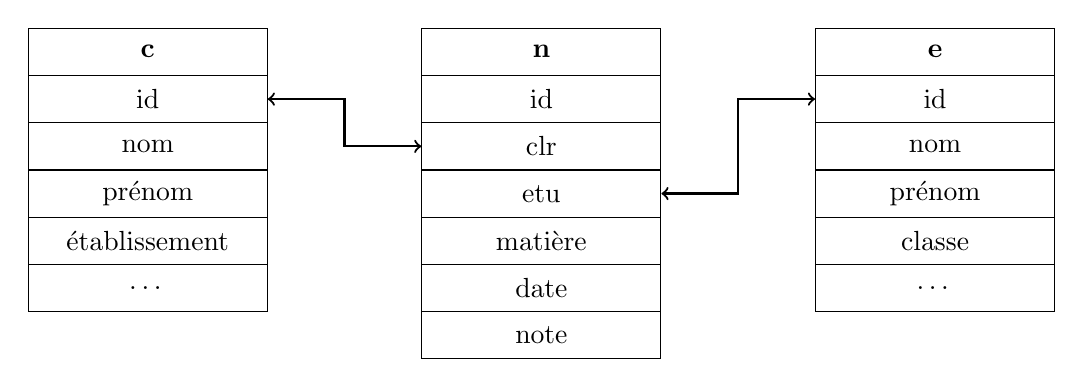
\begin{tikzpicture}
\node[table] at (-1, 0.0) {\bf c};
\node[table] at (-1,-0.6) (c-id) {id};
\node[table] at (-1,-1.2)        {nom};
\node[table] at (-1,-1.8)        {prénom};
\node[table] at (-1,-2.4)        {établissement};
\node[table] at (-1,-3.0)        {\dots};
\node[table] at ( 4, 0.0) {\bf n};
\node[table] at ( 4,-0.6)          {id};
\node[table] at ( 4,-1.2) (n-id-c) {clr};
\node[table] at ( 4,-1.8) (n-id-e) {etu};
\node[table] at ( 4,-2.4)          {matière};
\node[table] at ( 4,-3.0)          {date};
\node[table] at ( 4,-3.6)          {note};
\draw[thick, <->] (c-id) -- +(2.5,0) |- (n-id-c);
\node[table] at ( 9, 0.0) {\bf e};
\node[table] at ( 9,-0.6) (e-id) {id};
\node[table] at ( 9,-1.2)        {nom};
\node[table] at ( 9,-1.8)        {prénom};
\node[table] at ( 9,-2.4)        {classe};
\node[table] at ( 9,-3.0)        {\dots};
\draw[thick, <->] (e-id) -- +(-2.5,0) |- (n-id-e);
\end{tikzpicture}
\caption{Structure de la base de données}
\end{center}
\end{figure}
%--------------------------------------------------------------------------
\newpage
%--------------------------------------------------------------------------
\section{Utilisation de plusieurs tables}
%--------------------------------------------------------------------------
%--------------------------------------------------------------------------
\subsection{Produit}
%--------------------------------------------------------------------------
%--------------------------------------------------------------------------
Le premier moyen d'assembler deux relations est d'en faire le produit cartésien. 

On crée ainsi une nouvelle table en général beaucoup plus importante.
%--------------------------------------------------------------------------
\begin{defin}[Produit de deux relations]

Si $r$ est une relation de schéma $R$ et $r'$ est une relation de schéma $R'$ avec $R$ et $R'$ disjoints

alors le produit de $r$ et $r'$ est la relation $r\times r'$ de schéma $R\cup R'$ 

et dont l'extension est l'ensemble des fonctions définies sur $R\cup R'$ dont les restrictions à $R$ et à $R'$ appartiennent respectivement à l'extension de $r$ et à l'extension de $r'$.

L'abus usuel d'écriture donne
$r\times r'=\bigl\{u\ ;\ u[R]\in r,\ u[R']\in r'\bigr\}$
\end{defin}
%--------------------------------------------------------------------------

La condition $R\cap R'=\emptyset$ n'est pas très contraignante, il suffit de renommer les noms des attributs ; en général on notera {\bf r.xxx} tous les attributs de $r$ et {\bf r'.xxx} tous les attributs de $r'$ pour éviter les homonymies. En SQL, le produit est simplement engendré en listant les tables à multiplier dans la clause {\sc FROM} séparées par des virgules.

Par exemple le produit de $n$  et de $e$ revient à associer les notes de tout le monde avec chaque étudiant
%--------------------------------------------------------------------------
\begin{table}[ht]
\caption{Produit des tables : $n\times e$}
\begin{center}
\begin{tabular}{|c|c|c|c|c|c|c|c|c|c|c|c|}
\hline
{\bf n.id} &{\bf clr} &{\bf etu} & {\bf matière}&{\bf date} &{\bf heure} & {\bf note} &{\bf e.id} &{\bf nom} & {\bf prénom}&{\bf classe} & \dots\\
  \hline
1&2&1&Math&24/11/19&17h00&13&1&Aernout&Ludovic&PCSI1&\dots\\
1&2&1&Math&24/11/19&17h00&13&2&Camblor&Patricia&MPSI3&\dots\\
1&2&1&Math&24/11/19&17h00&13&3&Courbois&Éloïse&MP1&\dots\\
\dots&\dots&\dots&\dots&\dots&\dots&\dots&\dots&\dots&\dots\\
2&2&3&Math&24/11/19&13h00&17&1&Aernout&Ludovic&PCSI1&\dots\\
2&2&3&Math&24/11/19&13h00&17&2&Camblor&Patricia&MPSI3&\dots\\
\dots&\dots&\dots&\dots&\dots&\dots&\dots&\dots&\dots&\dots\\
\end{tabular}
\end{center}
\end{table}
%--------------------------------------------------------------------------

Pour des raisons d'encombrement on n'a écrit le préfixe que pour les colonnes de même nom. Dans la pratique il est recommandé de {\bf toujours} écrire le préfixe. 
%--------------------------------------------------------------------------
%--------------------------------------------------------------------------
\subsection{Produit amélioré}
%--------------------------------------------------------------------------
%--------------------------------------------------------------------------
Le produit ci-dessus ne représente rien sauf des paires note-étudiant. Si on veut vraiment les notes de colles pour chaque étudiant, on doit, dans le produit des tables $n$ et $e$, imposer la condition d'égalité des identifiants des étudiants. 
%--------------------------------------------------------------------------
\begin{lstlisting}[language=SQL]
SELECT e.nom, e.classe, n.matiere, n.date, n.note
FROM e, n
WHERE  e.id = n.edu
\end{lstlisting}
%--------------------------------------------------------------------------
Si on veut obtenir de plus le nom du colleur on doit utiliser les trois tables.
%--------------------------------------------------------------------------
\begin{lstlisting}[language=SQL]
SELECT e.nom, e.classe, c.nom, n.matiere, n.date, n.note
FROM c, e, n
WHERE  c.id = n.clr AND e.id = n.edu
\end{lstlisting}
%--------------------------------------------------------------------------
Bien entendu on peut ajouter des sélections. Les notes, avec le colleur, des étudiants de PCSI3 en chimie sont obtenues par 
%--------------------------------------------------------------------------
\begin{lstlisting}[language=SQL]
SELECT e.nom, e.classe, c.nom, n.matiere, n.date, n.note
FROM c, e, n
WHERE  c.id = n.clrAND e.id = n.edu
                     AND e.classe = "PCSI3"
                     AND n.matière = "Chim"
\end{lstlisting}
%--------------------------------------------------------------------------

%--------------------------------------------------------------------------
%--------------------------------------------------------------------------
\subsection{Jointure}
%--------------------------------------------------------------------------
%--------------------------------------------------------------------------
La réponse donnée ci-dessus n'est pas totalement satisfaisante : elle donne certes le bon résultat mais on écrit la requête en écrivant une sélection qui mélange une condition qui n'est pas facultative, celle provenant de la structure de la base, avec des critères de sélection qui dépendent de la question posée (clase, matière, \dots). 


La construction de la table produit ne contenant que les $n$-uplets respectant les conditions structurelles est donc fondamentale, c'est la {\bf jointure} (en fait equi-jointure).

%--------------------------------------------------------------------------
\begin{defin}[Jointure]

Si $r$ et $r'$ sont des relations et si $F$ est une condition sur $r\times r'$ 
alors la jointure de $r$ et $r'$ selon $F$ est la relation $r\bowtie_F r'=\sigma_F(r\times r')$.
\end{defin}
%--------------------------------------------------------------------------

La jointure n'apporte donc rien de nouveau quant aux résultats produits mais elle permet de mettre à des niveaux différents les critères de sélection selon qu'ils sont donnés par la structure ou simplement par la question posée.

La traduction de la jointure en SQL est
%--------------------------------------------------------------------------
\begin{lstlisting}[language=SQL]
table1 AS t1 JOIN table2 AS t2 ON t1.attribut1 = t2.attribut2
\end{lstlisting}
%--------------------------------------------------------------------------

On remarquera qu'on peut renommer les tables jointes afin de simplifier le nom des attributs quand on leur ajoute le nom de la table. L'exemple ci-dessus devient 
%--------------------------------------------------------------------------
\begin{lstlisting}[language=SQL]
SELECT e.nom, e.classe, n.matiere, n.date, n.note
FROM  e JOIN n ON e.id = n.edu
\end{lstlisting}
%--------------------------------------------------------------------------
{\bf Plusieurs jointures} : dans le cas de plusieurs tables, on a une condition de jointure à ajouter pour chaque nouvelle table. Par exemple pour les tables \type{table1}, \type{table2}et \type{table3}, on veut
\type{table1.attribut1 = table2.attribut2} et  \type{table1.attribut3 = table2.attribut4}.

On peut joindre les nouvelles tables à la jointure précédente
%--------------------------------------------------------------------------
\begin{lstlisting}[language=SQL]
table1 AS t1 JOIN table2 AS t2 ON t1.attribut1 = t2.attribut2
             JOIN table3 AS t3 ON t1.attribut3 = t3.attribut4
\end{lstlisting}
%--------------------------------------------------------------------------
ou joindre $n$ tables avec $n-1$conditions associées par {\sc and}.
%--------------------------------------------------------------------------
\begin{lstlisting}[language=SQL]
table1 AS t1 JOIN table2 AS t2 JOIN table3 AS t3 
             ON t1.attribut1 = t2.attribut2 AND t1.attribut3 = t3.attribut4
\end{lstlisting}
%--------------------------------------------------------------------------
\newpage
%--------------------------------------------------------------------------
\section{Exercices} 
%--------------------------------------------------------------------------
%--------------------------------------------------------------------------
Le type d'exercices donnés ici est celui que l'on retrouve dans les épreuves de concours : on doit écrire des requêtes sans pouvoir contrôler les résultats. En général, comme ici, on donne les schémas des tables et les relations qui servent aux jointures et quelques lignes d'exemples.

Les tables sont donc celles de la base de colle. On demande d'écrire les requêtes SQL qui permettent de donner les réponses aux questions.
%--------------------------------------------------------------------------
%--------------------------------------------------------------------------
\subsection{Requêtes simples} 
%--------------------------------------------------------------------------
%--------------------------------------------------------------------------
\begin{Exercise}
Quels sont les noms et prénoms des colleurs qui viennent du lycée Faidherbe ?
\end{Exercise}
%--------------------------------------------------------------------------
\begin{Answer}
\begin{lstlisting}[language=SQL]
SELECT nom, prénom
FROM c
WHERE établissement = "Faidherbe"
\end{lstlisting}
\end{Answer}
%--------------------------------------------------------------------------
%--------------------------------------------------------------------------
\begin{Exercise}
Quels sont les noms et prénoms des étudiants de la classe de MPSI4 ?
\end{Exercise}
%--------------------------------------------------------------------------
\begin{Answer}
\begin{lstlisting}[language=SQL]
SELECT nom, prénom
FROM e
WHERE classe = "MPSI4"
\end{lstlisting}
\end{Answer}
%--------------------------------------------------------------------------
%--------------------------------------------------------------------------
\begin{Exercise}
Quelles sont les matières qui ont eu au moins une colle le "07/12/19" ?
\end{Exercise}
%--------------------------------------------------------------------------
\begin{Answer}
\begin{lstlisting}[language=SQL]
SELECT DISTINCT matière
FROM n
WHERE date = "07/12/2019"
\end{lstlisting}
\end{Answer}
%--------------------------------------------------------------------------
%--------------------------------------------------------------------------
\subsection{Agrégations} 
%--------------------------------------------------------------------------
%--------------------------------------------------------------------------
\begin{Exercise}
Combien y-a-t-il d'élèves par classe ?
\end{Exercise}
%--------------------------------------------------------------------------
\begin{Answer}
\begin{lstlisting}[language=SQL]
SELECT classe, COUNT() AS nombre
FROM e
GROUP BY classe
\end{lstlisting}
\end{Answer}
%--------------------------------------------------------------------------
%--------------------------------------------------------------------------
\begin{Exercise}
Donner les note maximale, la note minimale et la moyenne des notes par matière.
\end{Exercise}
%--------------------------------------------------------------------------
\begin{Answer}
\begin{lstlisting}[language=SQL]
SELECT matière, MAX(note) AS note_max, MIN(note) AS note_min, AVG(note) AS note_moyenne
FROM n
GROUP BY matière
\end{lstlisting}
\end{Answer}
%--------------------------------------------------------------------------
%--------------------------------------------------------------------------
\begin{Exercise}
Déterminer le nombre d’occurrences de chaque note.
\end{Exercise}
%--------------------------------------------------------------------------
\begin{Answer}
\begin{lstlisting}[language=SQL]
SELECT note, COUNT() as nb_occ
FROM n
GROUP BY note
\end{lstlisting}
\end{Answer}
%--------------------------------------------------------------------------
%--------------------------------------------------------------------------
\begin{Exercise}
Quels sont les lycées d'où proviennent plus de 30 colleurs ?
\end{Exercise}
%--------------------------------------------------------------------------
\begin{Answer}
\begin{lstlisting}[language=SQL]
SELECT établissement, COUNT() as nb_colleurs
FROM c
GROUP BY établissement
HAVING nb_colleurs >= 30
\end{lstlisting}
\end{Answer}
%--------------------------------------------------------------------------
%--------------------------------------------------------------------------
\begin{Exercise}
Quelles sont les matières qui ont donné une moyenne des notes supérieure à 15 ?
\end{Exercise}
%--------------------------------------------------------------------------
\begin{Answer}
\begin{lstlisting}[language=SQL]
SELECT matière, AVG(note) as note_moy
FROM n
GROUP BY matière
HAVING note_moy > 15
\end{lstlisting}
\end{Answer}
%--------------------------------------------------------------------------
%--------------------------------------------------------------------------
\subsection{Requêtes imbriquées} 
%--------------------------------------------------------------------------
%--------------------------------------------------------------------------
\begin{Exercise}
Quelle est le nombre maximal d'élèves par classe .
\end{Exercise}
%--------------------------------------------------------------------------
\begin{Answer}
\begin{lstlisting}[language=SQL]
SELECT MAX(nombre)
FROM (SELECT classe, COUNT() AS nombre
      FROM e
      GROUP BY classe)
\end{lstlisting}
\end{Answer}
%--------------------------------------------------------------------------
%--------------------------------------------------------------------------
\begin{Exercise}
Quelle est la note de colle la plus attribuée ?
\end{Exercise}
%--------------------------------------------------------------------------
\begin{Answer}
\begin{lstlisting}[language=SQL]
SELECT note
FROM (SELECT note, COUNT() as nb_occ
      FROM n
      GROUP BY note)
WHERE note = (SELECT MAX(note)
              FROM (SELECT note, COUNT() as nb_occ
                    FROM n
                    GROUP BY note)
             )
\end{lstlisting}
\end{Answer}
%--------------------------------------------------------------------------
%--------------------------------------------------------------------------
\subsection{Jointures} 
%--------------------------------------------------------------------------
%--------------------------------------------------------------------------
\begin{Exercise}
Donner les notes attribuées par le colleur dont le nom est "de Boisseson".
\end{Exercise}
%--------------------------------------------------------------------------
\begin{Answer}
\begin{lstlisting}[language=SQL]
SELECT n.note
FROM n JOIN c ON n.clr= c.id
WHERE c.nom = "de Boisseson"
\end{lstlisting}
\end{Answer}
%--------------------------------------------------------------------------
%--------------------------------------------------------------------------
\begin{Exercise}
Quels sont les étudiants (nom, prénom) qui ont eu au moins une fois 20 en colle ?
\end{Exercise}
%--------------------------------------------------------------------------
\begin{Answer}
\begin{lstlisting}[language=SQL]
SELECT e.nom, e.prenom
FROM n JOIN e ON n.etu = e.id
WHERE n.note = 20
\end{lstlisting}
\end{Answer}
%--------------------------------------------------------------------------
%--------------------------------------------------------------------------
\begin{Exercise}
Quelles sont les matières évaluées en colle en MPSI1 ?
\end{Exercise}
%--------------------------------------------------------------------------
\begin{Answer}
\begin{lstlisting}[language=SQL]
SELECT DISTINCT n.matière
FROM n JOIN e ON n.etu = e.id
WHERE e.classe  = "MPSI1"
\end{lstlisting}
\end{Answer}
%--------------------------------------------------------------------------
%--------------------------------------------------------------------------
\begin{Exercise}
Quels sont les colleurs qui collent en PCSI2 ?
\end{Exercise}
%--------------------------------------------------------------------------
\begin{Answer}
\begin{lstlisting}[language=SQL]
SELECT c.nom, c.prenom
FROM n JOIN e ON n.etu = e.id
       JOIN c ON n.clr= c.id
WHERE c.classe = "PCSI2"
\end{lstlisting}
\end{Answer}
%--------------------------------------------------------------------------
%--------------------------------------------------------------------------
\begin{Exercise}
Quels sont les étudiants ayant eu une colle avec le colleur Stéphane Hoguet en MPSI3 ? 

On donnera aussi la date et la note.
\end{Exercise}
%--------------------------------------------------------------------------
\begin{Answer}
\begin{lstlisting}[language=SQL]
SELECT e.nom, e.prenom, n.date, n.note
FROM n JOIN e ON n.etu = e.id
       JOIN c ON n.clr= c.id
WHERE c.classe = "MPSI3" AND c.nom = "HOGUET" 
                         AND c.prénom = "Stéphane"
\end{lstlisting}
\newpage
\end{Answer}
%--------------------------------------------------------------------------
%--------------------------------------------------------------------------
\subsection{Jointures avec agrégation} 
%--------------------------------------------------------------------------
%--------------------------------------------------------------------------
\begin{Exercise}
Donner la moyenne des notes des colles de mathématiques (\type{Math}) des étudiants de la classe de MPSI2.
\end{Exercise}
%--------------------------------------------------------------------------
\begin{Answer}
\begin{lstlisting}[language=SQL]
SELECT e.nom, e.prenom, AVG(n.note)
FROM n JOIN e ON n.etu = e.id
group by e.id
WHERE e.classe = "MPSI2" AND n.matière = "Math"
\end{lstlisting}
On notera qu'on n'a pas affiché l'identifiant des étudiants.
\end{Answer}
%--------------------------------------------------------------------------
%--------------------------------------------------------------------------
\begin{Exercise}
Donner la note maximale donnée par les colleurs en physique  (\type{Phys}).
\end{Exercise}
%--------------------------------------------------------------------------
\begin{Answer}
\begin{lstlisting}[language=SQL]
SELECT c.nom, c.prenom, MAX(n.note)
FROM n JOIN c ON n.clr= c.id
WHERE n.matière = "Phys"
\end{lstlisting}
\end{Answer}
%--------------------------------------------------------------------------
%--------------------------------------------------------------------------
\begin{Exercise}
Quels étudiants n'ont eu que des notes supérieure à 15 en chimie (\type{Chim}) en PCSI1 ?
\end{Exercise}
%--------------------------------------------------------------------------
\begin{Answer}
\begin{lstlisting}[language=SQL]
SELECT e.nom, e.prenom
FROM n JOIN e ON n.etu = e.id
WHERE e.classe = "PCSI1" AND n.matière = "Chim"
HAVING MIN(n.note) >= 15
\end{lstlisting}
\end{Answer}
%--------------------------------------------------------------------------
%--------------------------------------------------------------------------
\begin{Exercise}
Quels sont les étudiants de MPSI1 qui ont une moyenne de notes de colles supérieure à la moyenne de la classe en mathématique et en physique ?
\end{Exercise}
%--------------------------------------------------------------------------
\begin{Answer}
\begin{lstlisting}[language=SQL]
SELECT c.nom, c.prenom
FROM n JOIN e ON n.etu = e.id
WHERE e.classe = "MPSI1" AND n.matière = "Math"
GROUP BY e.id
HAVING AVG(note) > (SELECT AVG(moy)
                    FROM (SELECT e.id, AVG(note) AS moy 
                          FROM n JOIN e ON n.etu = e.id
                          WHERE e.classe = "MPSI1" AND n.matière = "Math"
                          GROUP BY e.id)
                   )
                   
INTERSECT

SELECT c.nom, c.prenom
FROM n JOIN e ON n.etu = e.id
WHERE e.classe = "MPSI1" AND n.matière = "Phys"
GROUP BY e.id
HAVING AVG(note) > (SELECT AVG(moy)
                    FROM (SELECT e.id, AVG(note) AS moy 
                          FROM n JOIN e ON n.etu = e.id
                          WHERE e.classe = "MPSI1" AND n.matière = "Phys"
                          GROUP BY e.id)
                   )
\end{lstlisting}
\end{Answer}
%--------------------------------------------------------------------------
\newpage
%--------------------------------------------------------------------------
\section{Compléments} 
%--------------------------------------------------------------------------
%--------------------------------------------------------------------------
\subsection{Division relationnelle}
%--------------------------------------------------------------------------
%--------------------------------------------------------------------------
Il existe une fonction réciproque du produit, la division, dans l'algèbre relationnelle. 

C'est l'ensemble des tuples sur $R\setminus R'$ que l'on peut prolonger sur $R$ avec tous les tuples de $r'$ en obtenant toujours un tuple de $r$.

On a $(r \times r')\div r'=r$ et $(r \div r')\times r' \subset r$.
%--------------------------------------------------------------------------
\begin{defin}[Division de deux relations]

Si $r$ est une relation de schéma $R$ et $r'$ est une relation de schéma $R'$ avec $R'\subset R$ 

alors la division de $r$ par $r'$ est la relation $r \div r'$ de schéma $R\setminus R'$ dont l'extension est l'ensemble des $n$-uplets $l$ sur $R\setminus R'$ telles que, pour tout $n$-uplet $l'$ appartenant à l'extension de $r'$, l'union de $l$ et $l'$ appartient à l'extension de $r$..

L'abus usuel d'écriture donne
$r\div r'=\bigl\{u\ ;\ \forall t'\in r',\ (u,t')\in r\bigr\}$.
\end{defin}
%--------------------------------------------------------------------------
Il n'existe pas en SQL d'équivalent direct à la division.
%--------------------------------------------------------------------------
\subsubsection{Un exemple}
%--------------------------------------------------------------------------
On crée la table {\bf classe} des classes
%--------------------------------------------------------------------------
\begin{lstlisting}[language=SQL]
SELECT DISTINCT classe
FROM e
\end{lstlisting}
%--------------------------------------------------------------------------
On crée aussi la table {\bf recap} des colleurs et des classes qui les concernent
%--------------------------------------------------------------------------
\begin{lstlisting}[language=SQL]
SELECT DISTINCT c.nom, e.classe
FROM c JOIN n JOIN e 
       ON c.id = n.clr AND n.etu = e.id
\end{lstlisting}
%--------------------------------------------------------------------------
Le quotient {\bf recap $\div$ classe} est la table des colleurs qui collent dans {\bf toutes} les classes.

Voici une requête permettant d'obtenir le résultat.
%--------------------------------------------------------------------------
\begin{lstlisting}[language=SQL]
SELECT c.nom
FROM c JOIN n JOIN e 
       ON c.id = n.clrAND n.etu = e.id
GROUP BY c.id
HAVING COUNT(DISTINCT e.classe) = (SELECT  COUNT()
                                   FROM (SELECT DISTINCT classe FROM e)
                                  )
\end{lstlisting}
%--------------------------------------------------------------------------
{\bf Remarques}
\begin{itemize}
    \item L'agrégation porte sur \type{c.id} mais on n'affiche que \type{c.nom} qui est unique pour un identifiant donné.
    \item Le sélection avec \type{HAVING} utilise un calcul statistique qui n'est pas affiché.
    \item On a ajouté le modificateur \type{DISTINCT} qui permet de ne compter que les éléments distincts.
    \item On l'a utilisé aussi dans la projection \type{SELECT DISTINCT classe} car une table peut avoir des doublons en SQL, ce n'est pas ce qui est attendu en algèbre relationnelle.
\end{itemize}
%--------------------------------------------------------------------------
\newpage
%--------------------------------------------------------------------------
\subsection{Création de bases avec SQL} 
%--------------------------------------------------------------------------
%--------------------------------------------------------------------------
En complément nous allons présenter, sur l'exemple du chapitre, la création d'une base.

Il ne s'agit que d'une introduction, la création d'une base est un problème qui demande beaucoup d'attention et de savoir-faire.
%--------------------------------------------------------------------------
%--------------------------------------------------------------------------
\subsubsection{Création du schéma}
%--------------------------------------------------------------------------
%--------------------------------------------------------------------------
Pour créer une table il faut en énumérer les attributs en leur donnant un type. 

Les types les plus courants sont
%--------------------------------------------------------------------------
\begin{itemize}
\item INTEGER, un entier
%--------------------------------------------------------------------------
\item REAL, un réel
%--------------------------------------------------------------------------
\item CHAR(n), une chaîne de n caractères exactement
%--------------------------------------------------------------------------
\item VARCHAR(n), une chaîne de n caractères au plus
\end{itemize}
%--------------------------------------------------------------------------
Il faut aussi spécifier les composantes de la clé primaire. 

Cela se fait en écrivant les attributs de la clé primaire après les définitions des attributs. 
%--------------------------------------------------------------------------
\begin{lstlisting}[language=SQL]
CREATE TABLE xxx(
    ....
    PRIMARY KEY(attribut1, attribut2, ...));
\end{lstlisting}
Si la clé primaire ne contient qu'un attribut on peut le signaler lors de la définition.
%--------------------------------------------------------------------------
\begin{lstlisting}[language=SQL]
CREATE TABLE colleurs(
    id INTEGER PRIMARY KEY,
    nom VARCHAR(20),
    prénom VARCHAR(20),
    établissement VARCHAR(20);
\end{lstlisting}
%--------------------------------------------------------------------------
%--------------------------------------------------------------------------
\subsubsection{Clé étrangère}
%--------------------------------------------------------------------------
On peut ajouter une contrainte de clé étrangère par

\type{FOREIGN KEY (attribut) REFERENCES AutreTable (AutreTable.attribut)}

Lors d'usage d'une table avec clé étrangère, le logiciel de base de données se chargera de la  vérification de l'existence de la clé référencée
%--------------------------------------------------------------------------
\begin{lstlisting}[language=SQL]
CREATE TABLE n(
    id INTEGER PRIMARY KEY,
    clrINTEGER,
    etu INTEGER,
    matière VARCHAR(20),
    date VARCHAR(20),
    note INTEGER,
    FOREIGN KEY (id_c) REFERENCES c (id),
    FOREIGN KEY (edu) REFERENCES e (id));
\end{lstlisting}
%--------------------------------------------------------------------------
\subsubsection{Extension}
%--------------------------------------------------------------------------
On introduit les différents n-uplets par l'instruction \type{INSERT INTO nomTable}

suivie de \type{VALUE (valeur1, \dots, valeurp);}

\medskip

On peut rentrer plusieurs n-uplets à la fois en les séparant par des virgules.

Si l'ordre d'entrée des valeurs n'est pas celui de la définition des tables on doit préciser les colonnes après INTO nomTable.

%--------------------------------------------------------------------------
\begin{lstlisting}[language=SQL]
INSERT INTO e 
VALUE (1, "Aernout", "Ludovic", "PCSI1"),
      (2, "Camblor", "Patricia", "MPSI3");
\end{lstlisting}




